As we described earlier, in \namd{} GPU design all nonbonded work 
is offloaded to GPU since its computation is most intensive.
In code shown in ~\ref{gpu-cpu-assignment}, it is implemented by assigning computes to GPU so long as 
it has the types of Nonbonded*, which include NonbondedPair and
NonbondedSelf.  

%\begin{lstlisting}[float,frame=single,caption={Compute Assignment},label=gpu-cpu-assignment]
\begin{lstlisting}[frame=single,caption={Compute Assignment},label=gpu-cpu-assignment]
switch ( type of compute )    
{
    case computeNonbondedPairType:
            register_cuda_compute_pair(i,pid2,trans2);
            break
   ........................
   other types:
            create computes on CPU
            break;
}

\end{lstlisting}

\textbf{Motivation} : While this is a straightforward way to balance load between CPU and GPU, 
it may have significant performance problem depending on the configuration
of GPU and CPU.

We first did our experiments on two machines. The first is a multicore desktop with old GTX8800 
GPU and Intel Core2 Quad cores. The other machine is JYC, a test bed of Blue Waters. Each GPU node of 
JYC has 1 Kelper GPU and 16 AMD Interlagos cores. Table~\ref{tab:jac-desktop} shows the time step 
of simulating $23558-atom DHFR$ system on lab machine. It can be seen that the time step 
does not change when we use GPU or not. Moreover, using more CPU cores also does not help improve performance.
This is mainly because GPU is so slow and becomes the bottleneck of the performance.

\begin{table*}
\centering
\begin{tabular}{|c|c|c|c|}
\hline
 configuration & 1 CPU core  & 1 CPU core + 1 GPU & 4 CPU cores + 1 GPU \\
\hline
timestep (ms/step) & 673 & 725 & 720 \\
\hline 
\end{tabular}
\caption{Simulating 23558 atoms DHFR on desktop}
\label{tab:jac-desktop}
\end{table*}

Table~\ref{tab:jac-JYC} shows the time step of simulating $92224-atom Apoa1$
using one node of JYC. In the cases of using only one CPU core and one CPU core 
plus one GPU core, using GPU provides a speedup of 8.4x. 
Also when we increase the number of CPU cores upto 15, 
 the speedup is almost 40x.   

\begin{table*}
\centering
\begin{tabular}{|c|c|c|c|}
\hline
 configuration & 1 CPU core  & 1 CPU core + 1 GPU & 15 CPU cores + 1 GPU \\
\hline
timestep (ms/step) & 990 & 117 & 25 \\
\hline 
\end{tabular}
\caption{Simulating 92224 atoms Apoa1 using one node of JYC }
\label{tab:jac-JYC}
\end{table*}


To better understand the performance change in table~\ref{tab:jac-JYC},
we plot timelines of CPU and GPU execution. 
Fig.~\ref{figs:gpu-ppn1} and ~\ref{figs:gpu-ppn15} show the timeline of 
running $92,224$ atom Apoa1 using 1 GPU and 1 CPU core, 1GPU and 15 CPU cores.
Each main line represents execution on one CPU core. Different colors stand for 
different function execution. The red activity is for integration while the purple
is all bonded work on CPU. The white color stands for idle time. The green bars on top of the main bars 
show the execution of GPU. In Fig.~\ref{figs:gpu-ppn1}, the total time range 
is around $117 ms$, which is the time for one simulation step. We can see that
GPU only takes a small portion of total time, which is around $19 ms$.
In this case, it is correct that we should offload as much nonboned work as possible
to GPU since CPU execution is relatively slow. 

However, in Fig.~\ref{figs:gpu-ppn15} when we increase the number of CPU cores, 
the work on CPU side is parallelized and time is reduced to $12 ms $ while the GPU exection
still takes $19 ms$. As a result, on CPU side, there is a big portion of idle time.    

\begin{figure}[h]
\centering
\subfigure[1CPU core + 1 GPU] {\label{figs:gpu-ppn1}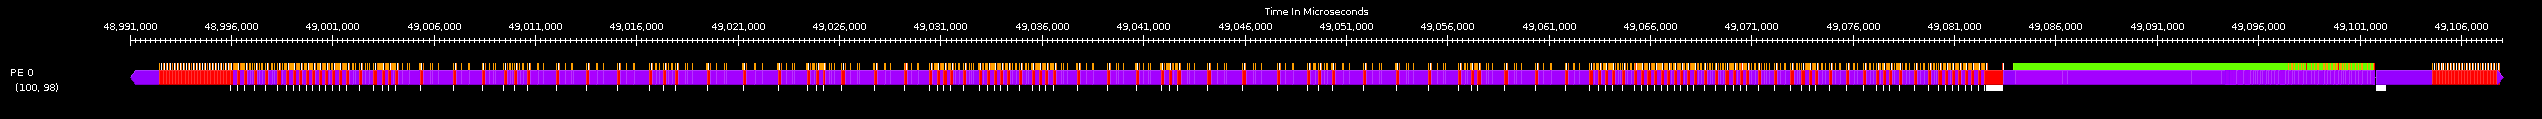
\includegraphics[width=5.8in]{figs/gpu-ppn1-timeline-117ms.png}}
\subfigure[15 CPU cores + 1 GPU] {\label{figs:gpu-ppn15}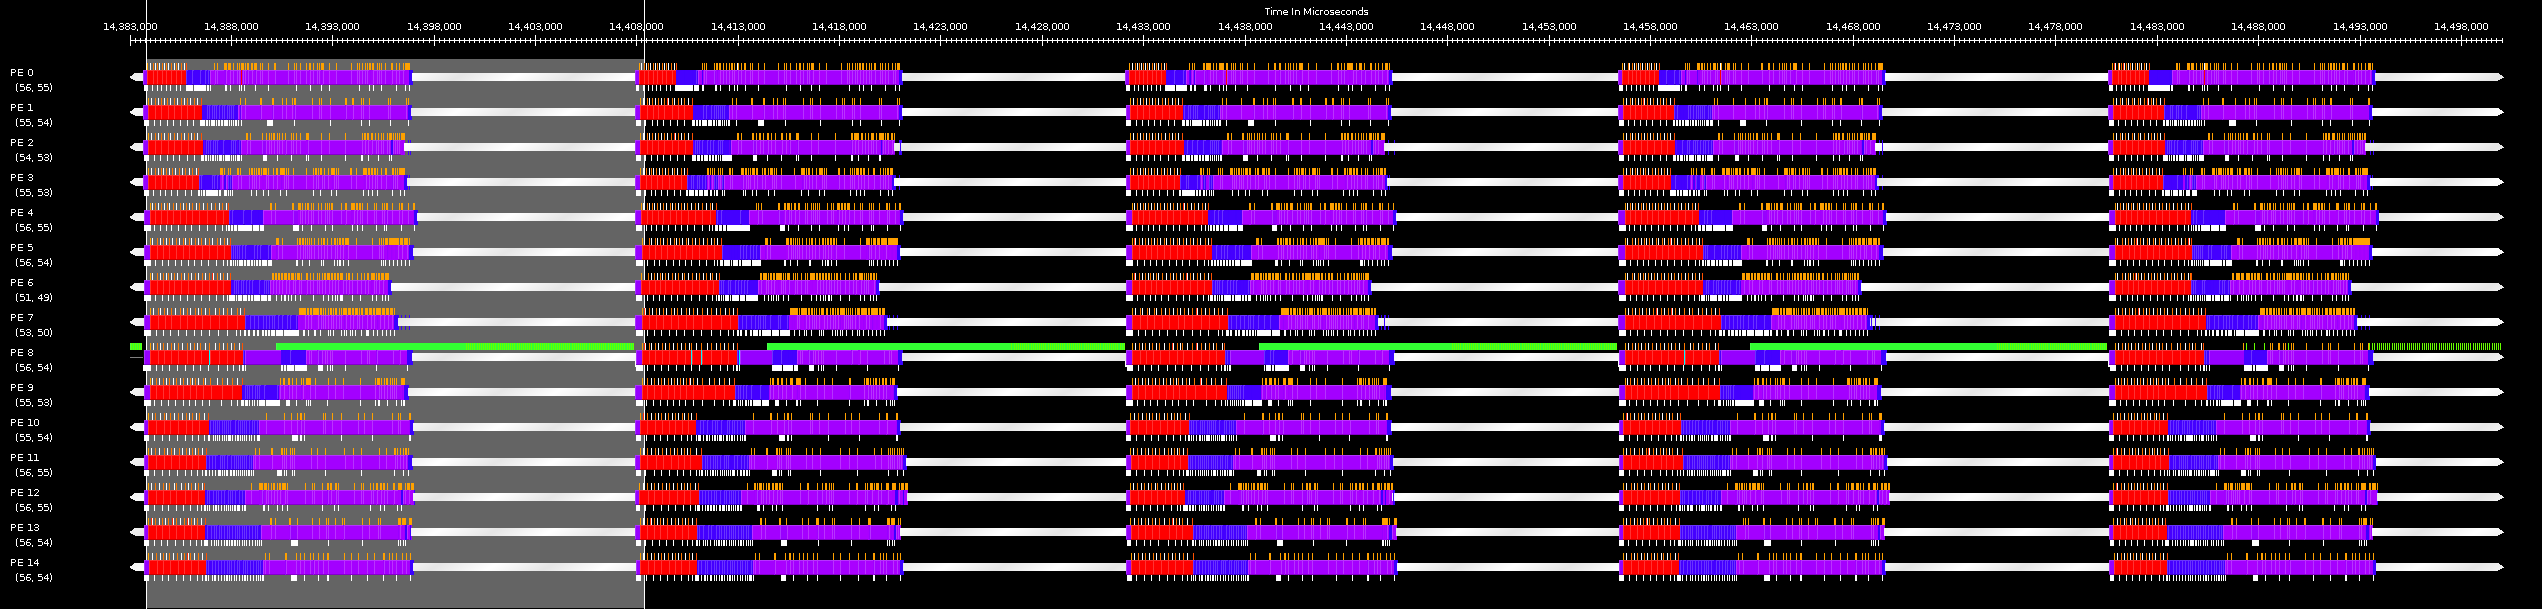
\includegraphics[width=5.8in]{figs/gpu-ppn15-timeline-117-25ms.png}}
\caption{Timeline of running Apoa1 with 1 GPU and different number of CPU cores}
\label{figs:cpu-gpu}
\end{figure}

\textbf{Load Balance} From table~\ref{tab:jac-desktop}, we can conclude that 
to calculate the same amount of nonboned work, the speed of GPU to CPU is 
$673:725 = 9:10$. Therefore, when one CPU core and one GPU is used, 
    the ratio of their nonboned work is roughly $10:9$. When using multiple CPU cores,
    the ratio of CPU and GPU work should be  $10*cores : 9 $.

In table~\ref{tab:jac-JYC}, when using one CPU core, the time to calculate nonboned work 
is  $ 990-117 = 873$. When all nonboned work is offload to GPU, the time cost is 
$18$ as shown in green bars in Fig.~\ref{figs:cpu-gpu}. Therefore, the ration of GPU 
and CPU capability is $873:18 = 48:1$. Since we have multiple CPU cores, the ratio of work on CPU 
and GPU should be $ Cores: 48 $.

Currently, we hard code this ratio into code. In future, we plan to use more intelligent instrumentation-based
balance scheme. Now with balance scheme, when we assign work, we need to figure out 
whether a compute should be placed on GPU or CPU. The changed code is as follow:

\begin{lstlisting}[frame=single,caption={Balanced Compute Assignment},label=gpu-cpu-assignment-balance]
switch ( type of compute )    
{
   case computeNonbondedPairType:
     if(computeid % ratio  < GPUload)
         register_cuda_compute_pair(i,map->computeData[i].pids[0].pid);
     else
     {
         c = new ComputeNonbondedPair(i,map->computeData[i].pids[0].pid,
             computeNonbondedWorkArrays,
             map->partition(i),map->partition(i)+1,
             map->numPartitions(i)); // unknown delete
            //assign work on CPU
            map->registerCompute(i,c);
            c->initialize();
       }
     break;

     other types:
         create computes on CPU
         break;
}
\end{lstlisting}
